%%%%%%%%%%%%%%%%%%%% chapter.tex (Chapter 2) %%%%%%%%%%%%%%%%%%%%%%%%%%%%%
% Chapter 2: Switching Techniques, Flow Control & Buffer Management
%%%%%%%%%%%%%%%%%%%%%%%%%%%%%%%%%%%%%%%%%%%%%%%%%%%%%%%%%%%%%%%%%%%%%%%%%

\chapter{Switching Techniques, Flow Control \& Buffer Management}
\label{ch:switching_flow_control}

\author{NoC-Lab Research Consortium}
\institute{NoC-Lab Research Consortium \at Shanghai Jiao Tong University \& International Collaborators, \email{research@network-on-chip.org}}

\maketitle

\abstract*{The efficiency, latency, and area footprint of an on-chip network are fundamentally dictated by its switching and flow control architecture. This chapter explores how raw application messages are decomposed into packets, flits, and phits, and details how silicon Network Interfaces bridge industry-standard protocols such as ARM AMBA AXI4 to internal NoC channels. We develop rigorous mathematical latency formulations comparing Store-and-Forward (SAF), Virtual Cut-Through (VCT), and Wormhole switching. We analyze lossless flow control mechanisms, proving the fundamental relationship between credit turnaround loop round-trip time (RTT) and minimum buffer sizing to sustain wire-rate throughput. Finally, we examine low-power alternative flow-control architectures, featuring the SWIFT token flow-control router with flit buffer bypassing.}

\abstract{The efficiency, latency, and area footprint of an on-chip network are fundamentally dictated by its switching and flow control architecture. This chapter explores how raw application messages are decomposed into packets, flits, and phits, and details how silicon Network Interfaces bridge industry-standard protocols such as ARM AMBA AXI4 to internal NoC channels. We develop rigorous mathematical latency formulations comparing Store-and-Forward (SAF), Virtual Cut-Through (VCT), and Wormhole switching. We analyze lossless flow control mechanisms, proving the fundamental relationship between credit turnaround loop round-trip time (RTT) and minimum buffer sizing to sustain wire-rate throughput. Finally, we examine low-power alternative flow-control architectures, featuring the SWIFT token flow-control router with flit buffer bypassing.}

\section{The Data Granularity Hierarchy: Messages, Packets, Flits \& Phits}
\label{sec:ch2_granularity}

Transmitting arbitrary software data structures across silicon requires decomposing raw application payloads into structured physical transmission units. To optimize buffer utilization, minimize pipeline latency, and guarantee deadlock-free routing, on-chip networks establish a four-layer data abstraction hierarchy: \textbf{Messages}, \textbf{Packets}, \textbf{Flits}, and \textbf{Phits}~\cite{Dally2001,Benini2002}.

\subsection{Architectural Motivation: Bridging the Semantic-Silicon Gap}
\label{subsec:ch2_granularity_motivation}

In traditional distributed computer networks and local-area networks (governed by the classical OSI or TCP/IP protocol stacks), communication spans meters or kilometers of physical cable. In such environments, physical pins and serial transceivers are scarce, transmission line delays are substantial, packet losses occur over noisy channels, and endpoint compute nodes possess gigabytes of cheap DRAM to buffer large, variable-length frames (e.g., standard Ethernet frames of 64 to 1,518~bytes).

On a monolithic silicon die or multi-die 2.5D/3D package, these physical trade-offs invert completely:
\begin{enumerate}
    \item \textbf{Buffer Area and Leakage Scarcity}: On-chip router buffers---implemented with dual-ported SRAM macros or D-flip-flop register files---consume between 35\% and 65\% of the total router silicon area and static leakage power~\cite{Dally2001,Fischer2025}. Dedicating tens of kilobytes of buffer storage per input port would severely cannibalize silicon budget from processing cores, vector units, and cache arrays.
    \item \textbf{Abundant On-Chip Wiring Density}: Modern deep-submicron and FinFET/GAAFET process nodes provide 10 to 16 back-end-of-line (BEOL) metal layers. While off-chip package pins remain tightly constrained, on-chip routers can deploy wide parallel buses (32 to 512 physical wires) across intermediate metal layers (M4--M6) with zero packaging penalty.
    \item \textbf{Sub-Nanosecond Single-Cycle Pipelining}: Packet switching, credit processing, virtual channel allocation, and crossbar traversal must execute in 1 to 2 clock cycles (300~ps to 1~ns), strictly precluding dynamic software intervention, complex variable-length frame reassembly, or multi-cycle header decoding.
\end{enumerate}

To reconcile these physical realities, Network-on-Chip (NoC) architectures partition data transmission across four distinct hierarchical boundaries, as summarized in Table~\ref{tab:ch2_granularity_taxonomy}.

\begin{table}[t]
\caption{The Four-Tier Data Granularity Hierarchy in Silicon Interconnects}
\label{tab:ch2_granularity_taxonomy}
\begin{tabular}{p{2.0cm}p{2.2cm}p{2.2cm}p{2.2cm}p{2.8cm}}
\hline\noalign{\smallskip}
Abstraction Level & Semantic Role & Operating Hardware & Allocation Horizon & Primary Architectural Constraints \\
\noalign{\smallskip}\svhline\noalign{\smallskip}
\textbf{Application Message} & Transaction semantics (coherence, DMA) & Core, L2/L3 Cache, Memory Controller & End-to-end transaction lifecycle & Unbounded length, bimodal traffic, protocol deadlock \\
\textbf{Packet} & Routing path \& deadlock freedom & Network Interface (NI), Router Routing Unit & Path traversal duration & Head-of-line blocking, routing deadlock, out-of-order delivery \\
\textbf{Flit (Flow Control Unit)} & Buffer allocation \& flow control credit & Router Virtual Channel (VC) Buffers & Hop-by-hop buffer credit loop & Silicon buffer area/leakage, credit turnaround round-trip time ($RTT$) \\
\textbf{Phit (Physical Unit)} & Physical clock-cycle signal transport & Physical Links, Repeaters, Crossbar & Single clock cycle edge & Wire pitch, crosstalk noise, Elmore $RC$ delay, clock skew \\
\noalign{\smallskip}\hline\noalign{\smallskip}
\end{tabular}
\end{table}

\subsection{The Four Abstraction Tiers and Functional Boundaries}
\label{subsec:ch2_four_tiers}

\subsubsection{Tier 1: Application Messages (The Transaction Semantic Unit)}
The \textbf{Application Message} is the software-level communication payload exchanged between processing cores, hardware accelerators (GPUs, TPUs, NPUs), and memory subsystem controllers (L2/L3 cache banks, HBM/DDR memory controllers). It encapsulates complete architectural semantics, including:
\begin{itemize}
    \item \textbf{Cache Coherence Invocations}: Short control messages such as Read Shared (\texttt{RdBlk}), Read Exclusive (\texttt{RdBlkMod}), Invalidate (\texttt{Inv}), or Writeback Acknowledgment (\texttt{WbAck}), typically spanning 8 to 16~bytes.
    \item \textbf{Cache Line Refills and Evictions}: 64-byte or 128-byte data payloads transferring an entire cache block between cache levels.
    \item \textbf{Direct Memory Access (DMA) Bursts}: Multi-kilobyte block transfers (e.g., 4~KB memory pages, large matrix weight tensors) generated by DMA engines or streaming accelerators.
\end{itemize}
Raw messages cannot be routed directly across the network fabric because their unbounded lengths would monopolize shared router buffers, triggering severe head-of-line (HOL) blocking and protocol-level deadlocks.

\subsubsection{Tier 2: Packets (The Architectural Routing Unit)}
The Network Interface (NI) decomposes or encapsulates application messages into one or more \textbf{Packets}. The packet constitutes the fundamental \emph{routing unit} of the network: all path routing algorithms (e.g., Dimension-Order Routing, Turn Models, or Valiant Oblivious Routing), virtual network isolation, and deadlock-avoidance proofs operate at the packet granularity.

A packet is formally defined as the tuple:
\begin{equation}
\mathcal{P} = \left\{ H_{\text{meta}},\, D_{\text{payload}},\, T_{\text{check}} \right\}
\label{eq:ch2_packet_tuple}
\end{equation}
where:
\begin{itemize}
    \item $H_{\text{meta}}$ denotes the routing header metadata, encompassing destination coordinates $(X_{\text{dest}}, Y_{\text{dest}}, Z_{\text{dest}})$, source address $(X_{\text{src}}, Y_{\text{src}})$, Virtual Network identifier ($VN_{\text{ID}}$), transaction identifier, quality-of-service (QoS) class, and packet length $L_{\text{pkt}}$.
    \item $D_{\text{payload}}$ is the data payload slice, constrained by the maximum transmission unit of the network ($MTU_{\text{noc}}$).
    \item $T_{\text{check}}$ is an optional integrity trailer (e.g., 16-bit CRC or parity checksum).
\end{itemize}

The \textbf{Packetization Framing Efficiency} ($\eta_{\text{pkt}}$) measures the fraction of transmitted bits dedicated to useful application data:
\begin{equation}
\eta_{\text{pkt}} = \frac{|D_{\text{payload}}|}{|H_{\text{meta}}| + |D_{\text{payload}}| + |T_{\text{check}}|} = \frac{|D_{\text{payload}}|}{B_{\text{pkt}}}
\label{eq:ch2_framing_efficiency}
\end{equation}
For a 64-byte cache line refill ($|D_{\text{payload}}| = 512$~bits) accompanied by a 32-bit header and 16-bit CRC ($B_{\text{pkt}} = 560$~bits), $\eta_{\text{pkt}} = \frac{512}{560} \approx 91.4\%$. Conversely, for an 8-byte cache coherence invalidation ($|D_{\text{payload}}| = 64$~bits), $\eta_{\text{pkt}} = \frac{64}{112} \approx 57.1\%$.

\begin{svgraybox}
\textbf{Why Routing Operates at Packet Granularity}:
Router Route Computation (RC) evaluates output port selection using combinational comparators or routing tables. If routing were evaluated per flit, every flit would require duplicate coordinate headers and pipeline stage overhead. Furthermore, flits belonging to different packets would interleave non-deterministically across physical links, causing corruption unless intermediate routers deployed expensive flit reassembly buffers. By enforcing packet-level routing, the leading flit establishes the path, and all subsequent flits trail along the reserved path without re-evaluating routing tables.
\end{svgraybox}

\subsubsection{Tier 3: Flow Control Units (Flits) (The Buffering and Allocation Unit)}
A packet is segmented into a sequenced stream of \textbf{Flow Control Units (Flits)}. The flit is the fundamental \emph{atomic unit of buffer storage allocation and flow control credit accounting}.

Router input buffers, virtual channels (VCs), and credit counters track resources exclusively in integer multiples of flits. Flits are partitioned into four distinct microarchitectural types:
\begin{enumerate}
    \item \textbf{Head Flit (\texttt{Flit\_Type = 2'b01})}:
    The opening flit of a multi-flit packet. It encapsulates the routing header ($H_{\text{meta}}$), destination coordinates, and priority. The Head flit arbitrates for downstream Virtual Channels during the Virtual Channel Allocation (VA) pipeline stage and reserves the routing state in intermediate routers.
    \item \textbf{Body Flits (\texttt{Flit\_Type = 2'b00})}:
    Intermediate flits carrying pure data payload. Body flits do not contain destination coordinates; they follow the virtual channel reservation established by their preceding Head flit. This eliminates redundant routing calculations and conserves dynamic pipeline switching power.
    \item \textbf{Tail Flit (\texttt{Flit\_Type = 2'b10})}:
    The terminal flit of a multi-flit packet. It carries the final payload fragment and optional error checksum ($T_{\text{check}}$). Crucially, as the Tail flit traverses the crossbar and departs an output port, it triggers the router control logic to \textbf{deallocate the Virtual Channel} and release channel state registers, returning the downstream VC state to \texttt{IDLE}.
    \item \textbf{Head-Tail Flit (\texttt{Flit\_Type = 2'b11})}:
    A single-flit packet ($L = 1$) combining header metadata, payload, and termination markers within a single clock cycle. This format is vital for short coherence transactions (invalidations, acknowledgments, credit returns), enabling single-cycle channel allocation and deallocation without serialization penalty.
\end{enumerate}

Let $W_{\text{flit}}$ denote the total flit width in bits, $W_{\text{ctrl}}$ denote the control field overhead per flit (e.g., 2-bit flit type and $v$-bit Virtual Channel ID), and $W_{\text{flit\_payload}} = W_{\text{flit}} - W_{\text{ctrl}}$ denote payload capacity. If the Head flit allocates $W_{\text{head\_hdr}}$ bits for destination coordinates and transaction tags, leaving $W_{\text{head\_payload}} = W_{\text{flit\_payload}} - W_{\text{head\_hdr}}$ for payload, the total packet length $L$ in flits is:
\begin{equation}
L = 1 + \left\lceil \frac{\max\left(0,\, |D_{\text{payload}}| + |T_{\text{check}}| - W_{\text{head\_payload}}\right)}{W_{\text{flit\_payload}}} \right\rceil
\label{eq:ch2_flit_decomposition}
\end{equation}
When the Head flit carries purely routing metadata ($W_{\text{head\_payload}} = 0$), this simplifies to:
\begin{equation}
L = 1 + \left\lceil \frac{|D_{\text{payload}}| + |T_{\text{check}}|}{W_{\text{flit\_payload}}} \right\rceil
\label{eq:ch2_flit_decomp_pure}
\end{equation}

\subsubsection{Tier 4: Physical Units (Phits) (The Clock-Cycle Signaling Unit)}
The \textbf{Physical Unit (Phit)} is the exact number of physical bits transferred across an inter-router link in \textbf{exactly one clock cycle}. The phit width equals the physical width of the physical link bus, $W_{\text{link}}$ (i.e., the count of conductive copper traces spanning between adjacent router ports).

The relationship between logical flits and physical phits is defined by the \textbf{Link Serialization Ratio} ($S$):
\begin{equation}
S = \left\lceil \frac{W_{\text{flit}}}{W_{\text{link}}} \right\rceil
\label{eq:ch2_serialization_ratio}
\end{equation}
The physical link latency per flit is given by $t_{\text{link}} = S \cdot t_{\text{cycle}}$. Three architectural regimes exist:
\begin{itemize}
    \item \textbf{Unserialized Transport ($S = 1$, $W_{\text{link}} = W_{\text{flit}}$)}: 1~Flit = 1~Phit. The complete flit traverses the link in a single clock cycle. This maximizes link throughput, eliminates serialization delay, and eliminates the need for input/output gearbox registers.
    \item \textbf{Sub-Flit Serialization ($S > 1$, $W_{\text{link}} < W_{\text{flit}}$)}: A flit is time-multiplexed across $S$ consecutive clock cycles over a narrower physical bus (e.g., a 128-bit flit transmitted across a 32-bit physical link incurs $S = 4$~cycles/flit). While this reduces metal wiring track congestion and crossbar area by factor $S$, it inflates link transit latency by $(S - 1)$ cycles per flit and requires serializer/deserializer (gearbox) register logic.
    \item \textbf{Ultra-Wide Interconnects ($W_{\text{link}} \ge 512$~bits)}: Modern high-throughput accelerators and open-source architectures like \textbf{FlooNoC}~\cite{Fischer2025} leverage upper metal layers to implement 512-bit physical links, matching an entire 64-byte cache line refill in a single flit and phit ($S = 1, L = 1$), completely eliminating multi-flit packet reassembly.
\end{itemize}

\subsection{Microarchitectural Flit Anatomy and Field Encoding}
\label{subsec:ch2_flit_anatomy}

Figure~\ref{fig:ch2_flit_formats} illustrates the canonical bitfield layout for on-chip flits in modern virtual-channel architectures.

\begin{figure}[t]
\centering
\begin{minipage}{0.98\textwidth}
\begin{verbatim}
HEAD FLIT (Routing & Channel Allocation):
+----------+--------+-----------+-------------+-------+-------+---------+----------+----------+
|Type (2b) |VC (3b) |Dest (8b)  |Lookahead(3b)|VN (2b)|QoS(2b)|Len (6b) |Trans(6b) |Data (32b)|
+----------+--------+-----------+-------------+-------+-------+---------+----------+----------+

BODY FLIT (Pure Payload Streaming):
+----------+--------+--------------------------------------------------------------+----------+
|Type (2b) |VC (3b) |-------------------- Raw Payload Data (57b) ------------------|Parity(2b)|
+----------+--------+--------------------------------------------------------------+----------+

TAIL FLIT (Packet Teardown & Checksum):
+----------+--------+-----------------------+--------------------------------------+----------+
|Type (2b) |VC (3b) | CRC / Checksum (16b)  |---------- Final Payload (41b) -------|Parity(2b)|
+----------+--------+-----------------------+--------------------------------------+----------+

HEAD-TAIL FLIT (Atomic Single-Flit Packet):
+----------+--------+-----------+-------------+-------+----------------------------+----------+
|Type (2b) |VC (3b) |Dest (8b)  |Lookahead(3b)|VN (2b)|---- Short Payload (40b) ---| CRC (12b)|
+----------+--------+-----------+-------------+-------+----------------------------+----------+
\end{verbatim}
\end{minipage}
\caption{Canonical microarchitectural flit bitfield encodings in modern virtual-channel NoCs: (a) Head flit with lookahead routing and transaction metadata, (b) Body flit with payload streaming, (c) Tail flit with integrity checksum, and (d) Head-Tail single-flit packet for low-latency coherence transactions.}
\label{fig:ch2_flit_formats}
\end{figure}

Key microarchitectural fields include:
\begin{itemize}
    \item \textbf{\texttt{Flit\_Type} (2~bits)}: Differentiates Body (\texttt{2'b00}), Head (\texttt{2'b01}), Tail (\texttt{2'b10}), and Head-Tail (\texttt{2'b11}) formats.
    \item \textbf{\texttt{VC\_ID} (2--4~bits)}: Directs incoming flits to the appropriate Virtual Channel buffer FIFO at the receiver port.
    \item \textbf{\texttt{Dest\_Coord} (8--12~bits)}: Encodes destination coordinates $(X_{\text{dest}}, Y_{\text{dest}}, Z_{\text{dest}})$ for routing logic.
    \item \textbf{\texttt{Lookahead\_Routing} (3~bits)}: In advanced low-latency routers~\cite{Peh2001}, the upstream router pre-computes the routing decision for the \emph{next downstream hop} and writes this direction (East, West, North, South, Local) into the Head flit. The downstream router reads this field immediately, allowing Virtual Channel Allocation (VA) and Switch Allocation (SA) to proceed in parallel with buffer write, shrinking zero-load router pipeline latency from 3--4 cycles down to a single cycle.
    \item \textbf{\texttt{VN\_ID} (2~bits)}: Virtual Network identifier used to segregate request, response, and coherence invalidation streams to guarantee protocol-level deadlock freedom.
    \item \textbf{\texttt{QoS\_Priority} (2~bits)}: Differentiates latency-sensitive control traffic from bulk throughput traffic.
    \item \textbf{\texttt{Trans\_ID} (6--8~bits)}: Unique transaction identifier mapped to Network Interface Reorder Buffers (RoBs).
\end{itemize}

\subsection{Architectural Walkthrough: Slicing a 64-Byte Cache Line Refill}
\label{subsec:ch2_walkthrough}

To concretize the interaction between the four abstraction tiers, consider an L1 data cache miss on Core $(0, 0)$ requesting a 64-byte ($512\text{ bits}$) cache line from an L2 cache bank at tile $(3, 3)$ across a 2D mesh:
\begin{enumerate}
    \item \textbf{Message Tier}: The L2 controller generates a 64-byte Read Response message containing the 512-bit cache line and a 32-bit transaction status header ($544\text{ bits}$ total).
    \item \textbf{Packet Tier}: The Network Interface encapsulates the message into a Response Packet. It prepends a 32-bit routing header ($H_{\text{meta}}$: destination $(0,0)$, source $(3,3)$, $VN = \text{Response}$, TransID $= 42$) and appends a 16-bit CRC checksum ($T_{\text{check}}$). Total packet size $B_{\text{pkt}} = 32 + 512 + 16 = 560\text{ bits}$. The framing efficiency is $\eta_{\text{pkt}} = \frac{512}{560} = 91.4\%$.
    \item \textbf{Flit Tier}: The packet is segmented into flits according to the microarchitecture's flit width $W_{\text{flit}}$. Table~\ref{tab:ch2_cache_refill_comparison} compares three standard NoC design points.
    \item \textbf{Phit Tier}: Flits are clocked onto physical wire links. Under a balanced 128-bit NoC, each 128-bit flit constitutes 1 phit ($S = 1$). The 5-flit packet traverses each inter-router link in 5 clock cycles, requiring a minimum downstream buffer depth of $B \ge 5$~flits to prevent cut-through stalling.
\end{enumerate}

\begin{table}[t]
\caption{Microarchitectural Comparison of a 64-Byte Cache Line Refill across NoC Configurations}
\label{tab:ch2_cache_refill_comparison}
\begin{tabular}{p{2.6cm}p{2.6cm}p{2.8cm}p{2.8cm}}
\hline\noalign{\smallskip}
Metric / Parameter & Config A (Narrow 64-bit) & Config B (Balanced 128-bit) & Config C (Wide 512-bit) \\
\noalign{\smallskip}\svhline\noalign{\smallskip}
Flit Width ($W_{\text{flit}}$) & 64 bits & 128 bits & 576 bits (512b data + 64b hdr) \\
Link Width ($W_{\text{link}}$) & 64 bits & 128 bits & 576 bits \\
Serialization Ratio ($S$) & 1 Phit/Flit & 1 Phit/Flit & 1 Phit/Flit \\
Flit Composition ($L$) & 10 flits (1 H, 8 B, 1 T) & 5 flits (1 H, 3 B, 1 T) & 1 flit (1 Head-Tail) \\
Channel Busy Duration & 10 clock cycles & 5 clock cycles & 1 clock cycle \\
Downstream Buffer Sizing & $\ge 10$ flits ($640\text{ bits}$) & $\ge 5$ flits ($640\text{ bits}$) & $\ge 1$ flit ($576\text{ bits}$) \\
Crossbar Area Scaling & Baseline ($1.0\times$) & $2.0\times$ baseline & $9.0\times$ baseline \\
Head-of-Line Contention & High (10 cycles/pkt) & Moderate (5 cycles/pkt) & Minimal (1 cycle/pkt) \\
\noalign{\smallskip}\hline\noalign{\smallskip}
\end{tabular}
\end{table}

\subsection{Silicon Trade-Offs: Wide vs. Narrow Interconnect Datapaths}
\label{subsec:ch2_wire_tradeoffs}

Choosing the boundary between flit width $W_{\text{flit}}$ and link width $W_{\text{link}}$ represents one of the most critical trade-offs in on-chip interconnection design:
\begin{enumerate}
    \item \textbf{Routing Congestion and Metal Layer Stack}:
    A 512-bit bidirectional physical link requires $2 \times 512 = 1,024$ physical wires. With an intermediate metal pitch (M4--M6) of $80\,\mathrm{nm}$, routing 1,024 wires consumes $\approx 82\,\mu\mathrm{m}$ of silicon routing width per router tile. If wire pitch cannot accommodate this density, designers must either insert multiplexed narrow links ($S > 1$) or dedicate upper global metal layers (M7--M9) with relaxed pitches and thick low-resistance copper traces.
    \item \textbf{Crosstalk and Dynamic Wire Energy}:
    Running hundreds of parallel wires in close proximity creates severe inter-wire coupling capacitance ($C_c$). When adjacent lines toggle in opposite directions, the effective Miller capacitance doubles ($C_{\text{eff}} = C_g + 2C_c$), inducing signal delay jitter. To preserve signal integrity at gigahertz clock rates, wide links often interleave ground shield wires (\texttt{GND-Signal-Signal-GND}), increasing effective wire track consumption by 30\% to 50\%.
    \item \textbf{Crossbar Switch Complexity}:
    The silicon area of a $P$-port crossbar switch scales quadratically with port count $P$ and linearly with flit width $W_{\text{flit}}$:
    \begin{equation}
    \text{Area}_{\text{xbar}} \approx P^2 \cdot W_{\text{flit}} \cdot A_{\text{crosspoint}}
    \label{eq:ch2_xbar_area}
    \end{equation}
    where $A_{\text{crosspoint}}$ is the standard-cell area of a single multiplexer bit-cell. Doubling flit width doubles crossbar area and input buffer registers, but halves packet length $L$, reducing channel occupancy time and queuing contention.
    \item \textbf{Wire Energy Efficiency}:
    Counterintuitively, wide parallel links often deliver superior energy efficiency compared to high-frequency serialized links. A wide 512-bit link operating at a conservative $1.0\,\mathrm{GHz}$ eliminates power-dense phase-locked loops (PLLs) and serializer/deserializer (SerDes) transceivers, achieving energy consumption as low as $0.15\,\mathrm{pJ/Byte/hop}$ ($0.019\,\mathrm{pJ/bit/hop}$) in modern FinFET processes~\cite{Fischer2025}.
\end{enumerate}

\section{Silicon Network Interface: The AXI4 / NoC Protocol Translation}
\label{sec:ch2_network_interface}

At the boundary between processing cores and the on-chip network fabric, the \textbf{Network Interface (NI)} bridges SoC protocol standards (such as ARM AMBA AXI4, OCP, or RISC-V TileLink) to the internal packetized NoC protocol.

\begin{figure}[t]
\centering
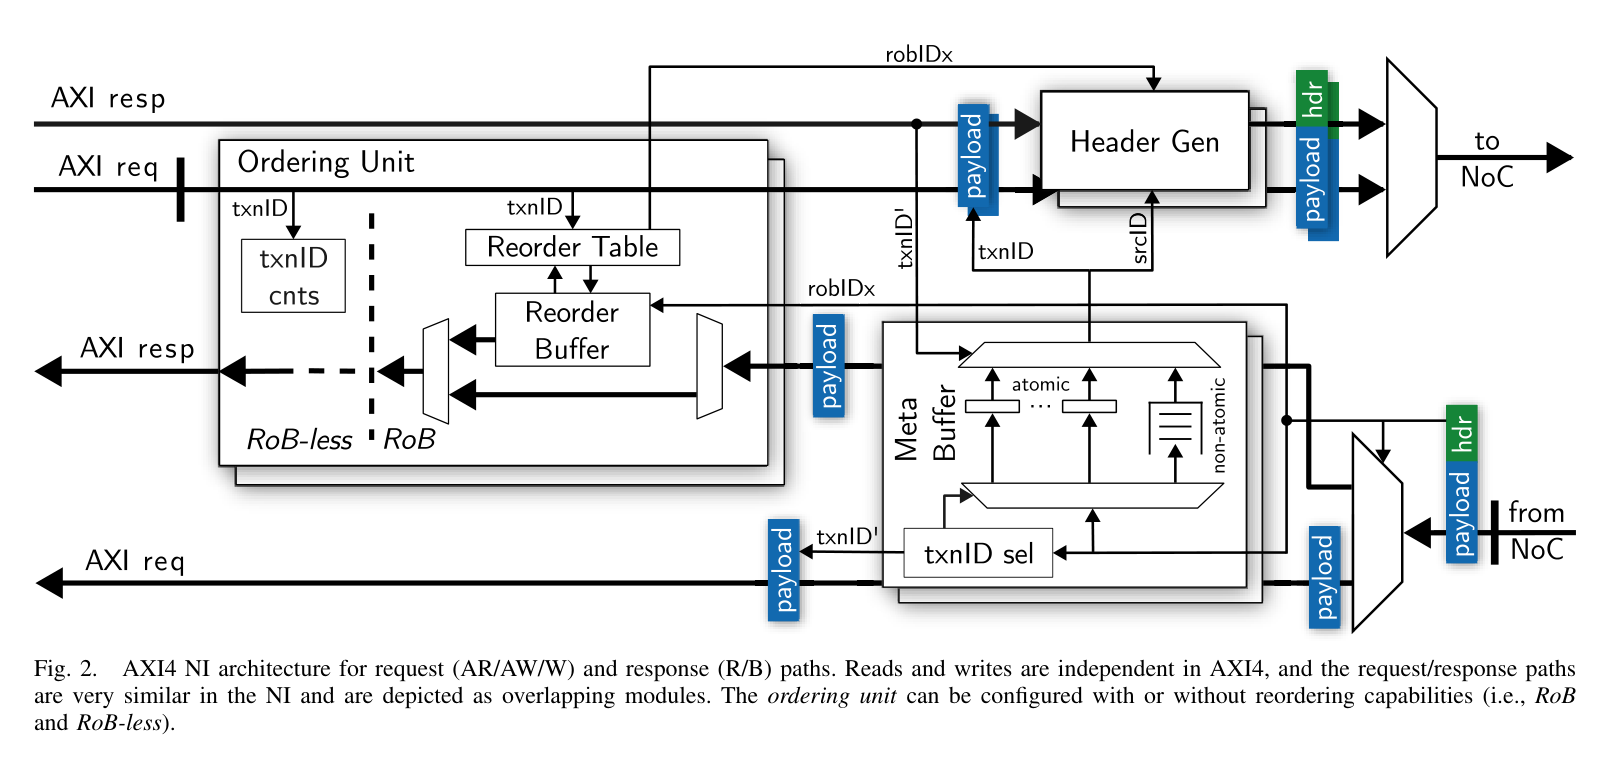
\includegraphics[width=0.88\textwidth]{chapters/ch02-switching-flow-control/figures/floonoc_fig02_axi_ni.png}
\caption{AXI4 Network Interface (NI) architecture for independent request (AR/AW/W) and response (R/B) paths, with reorder buffering (RoB) and direct DMA streaming. [Reproduced from: T. Fischer, M. Rogenmoser, T. Benz, F. K. G{\"u}rkaynak, and L. Benini, ``FlooNoC: A 645-Gb/s/link 0.15-pJ/B/hop Open-Source NoC With Wide Physical Links and End-to-End AXI4 Parallel Multistream Support,'' \emph{IEEE Trans. Very Large Scale Integr. (VLSI) Syst.}, vol. 33, no. 4, pp. 1094--1107, Apr. 2025~\cite{Fischer2025}. \copyright~2025 IEEE]}
\label{fig:ch2_floonoc_ni}
\end{figure}

As demonstrated in \textbf{FlooNoC}~\cite{Fischer2025}, modern high-performance NIs decouple independent AXI4 channels onto dedicated physical or virtual networks to prevent protocol-level deadlock:
\begin{itemize}
    \item \textbf{Request Network}: Translates Read Address (\texttt{AR}), Write Address (\texttt{AW}), and Write Data (\texttt{W}) channels into multi-flit request packets.
    \item \textbf{Response Network}: Translates Read Data (\texttt{R}) and Write Response (\texttt{B}) channels into separate response packets.
    \item \textbf{Reorder Buffer (RoB)}: Restores in-order AXI transaction completion when packets traverse adaptive, out-of-order routing paths.
\end{itemize}

\section{Mathematical Latency Analysis of Switching Techniques}
\label{sec:ch2_switching_analysis}

The switching technique dictates when and how an incoming flit is forwarded from an input port to an output port. We analyze three classical switching paradigms across path length $H$ (in hops), packet length $L$ (in flits), physical link bandwidth $W$ (bits/cycle), and router pipeline latency $t_r$ (cycles/hop).

\subsection{Store-and-Forward (SAF) Switching}
In Store-and-Forward switching, a router must receive, buffer, and verify the \emph{entire packet} before forwarding its first flit to the downstream router:
\begin{equation}
t_{serial} = \frac{L}{W}, \qquad T_{SAF} = H \cdot \left( t_r + \frac{L}{W} + t_{link} \right)
\label{eq:saf_latency}
\end{equation}
If $t_r + t_{link} \ll \frac{L}{W}$, the zero-load latency scales as:
\begin{equation}
T_{SAF} \approx H \cdot \frac{L}{W} \propto H \cdot L
\end{equation}
This multiplicative dependence ($H \cdot L$) imposes severe latency penalties over long distances and necessitates massive SRAM buffers ($\ge L$ flits per port).

\subsection{Virtual Cut-Through (VCT) Switching}
Introduced by Kermani \& Kleinrock~\cite{Kermani1979}, Virtual Cut-Through permits a router to forward the Head flit to the downstream router \emph{immediately} after route computation and arbitration, without awaiting trailing flits, provided the downstream router has allocated full packet buffer space:
\begin{equation}
T_{VCT} = H \cdot (t_r + t_{link}) + \frac{L - 1}{W}
\label{eq:vct_latency}
\end{equation}
Here, distance $H$ and packet length $L$ are \textbf{additive} ($H + L$), cutting zero-load latency dramatically under low traffic. However, VCT still requires allocating a full packet's worth of buffering ($B \ge L$) before granting admission.

\subsection{Wormhole (WH) Switching}
Proposed by Dally \& Seitz~\cite{Dally1987}, \textbf{Wormhole Switching} decouples flow control units from packet size:
\begin{svgraybox}
\textbf{The Wormhole Principle}: Router buffers operate at the granularity of individual \textbf{flits}, rather than entire packets. Buffer depth per virtual channel can be as small as 1 to 4 flits, completely independent of packet length $L$.
\end{svgraybox}

The zero-load latency of Wormhole switching mirrors VCT under uncongested conditions:
\begin{equation}
T_{WH} = H \cdot (t_r + t_{link}) + \frac{L - 1}{W}
\label{eq:wh_latency}
\end{equation}
However, the silicon area savings are transformative: router input buffers shrink by 75\% to 93\% compared to SAF and VCT, as demonstrated in Table~\ref{tab:switching_comparison}.

\begin{table}[t]
\caption{Analytical Comparison of Switching Techniques across 8 Hops ($t_r = 2$ cycles, $t_{link} = 1$ cycle)}
\label{tab:switching_comparison}
\begin{tabular}{p{1.8cm}p{1.6cm}p{1.8cm}p{1.8cm}p{2.0cm}p{2.2cm}}
\hline\noalign{\smallskip}
Packet Length & Hop Count & SAF Latency & VCT / WH Latency & Speedup of VCT/WH & Wormhole Buffer Area Saving \\
\noalign{\smallskip}\svhline\noalign{\smallskip}
4 flits  & 4 hops & 28 cycles  & 15 cycles & $1.87\times$ & Baseline \\
8 flits  & 4 hops & 44 cycles  & 19 cycles & $2.32\times$ & 50.0\% saving \\
16 flits & 4 hops & 76 cycles  & 27 cycles & $2.81\times$ & 75.0\% saving \\
32 flits & 4 hops & 140 cycles & 43 cycles & $3.26\times$ & 87.5\% saving \\
16 flits & 8 hops & 152 cycles & 39 cycles & $3.90\times$ & 75.0\% saving \\
32 flits & 8 hops & 280 cycles & 55 cycles & $5.09\times$ & 87.5\% saving \\
64 flits & 8 hops & 536 cycles & 87 cycles & $6.16\times$ & 93.8\% saving \\
\noalign{\smallskip}\hline\noalign{\smallskip}
\end{tabular}
\end{table}

\section{Queuing Theory Foundations of On-Chip Buffering}
\label{sec:ch2_queuing_theory}

To model buffer sizing, queue delays, and throughput saturation under stochastic traffic, we apply classical Markovian and deterministic queuing theory to on-chip router input channels.

\subsection{The $M/M/1/B$ and $M/D/1/B$ Finite Queue Models}
\label{subsec:ch2_finite_queue}

Consider an input virtual channel buffer of finite capacity $B$ flits. Packets arrive according to a Poisson process with average injection rate $\lambda$ (flits/cycle), and the crossbar switch services flits at service rate $\mu$ (flits/cycle). The traffic intensity (channel utilization factor) is defined as:
\begin{equation}
\rho = \frac{\lambda}{\mu}
\label{eq:ch2_rho}
\end{equation}

For an $M/M/1/B$ finite birth-death queuing process, the steady-state probability $p_k$ that exactly $k$ flits occupy the buffer ($0 \le k \le B$) satisfies the geometric progression:
\begin{equation}
p_k = \frac{(1 - \rho) \cdot \rho^k}{1 - \rho^{B+1}} \quad (\text{for } \rho \ne 1), \qquad p_k = \frac{1}{B + 1} \quad (\text{for } \rho = 1)
\label{eq:ch2_steady_state_pk}
\end{equation}

In a lossless on-chip network with backpressure, when the buffer is completely full ($k = B$), the upstream transmitter is blocked from injecting new flits. The probability of backpressure assertion (upstream stall) is:
\begin{equation}
P_{stall} = p_B = \frac{(1 - \rho) \cdot \rho^B}{1 - \rho^{B+1}}
\label{eq:ch2_p_stall}
\end{equation}

The average number of flits residing in the input queue, $N_{avg}$, is:
\begin{equation}
N_{avg} = \sum_{k=0}^{B} k \cdot p_k = \frac{\rho}{1 - \rho} - \frac{(B + 1) \cdot \rho^{B+1}}{1 - \rho^{B+1}}
\label{eq:ch2_navg}
\end{equation}

By Little's Law ($N_{avg} = \lambda_{eff} \cdot W_{queue}$), the average waiting time spent in the router buffer before crossbar traversal is:
\begin{equation}
W_{queue} = \frac{N_{avg}}{\lambda \cdot (1 - P_{stall})} = \frac{1}{\mu(1 - \rho)} - \frac{B \cdot \rho^B}{\mu (1 - \rho^B)}
\label{eq:ch2_wqueue}
\end{equation}

Under deterministic service ($\mu = 1.0$ flit/cycle when granted, modeled as an $M/D/1/B$ queue), queueing delay remains minimal for $\rho \le 0.60\text{--}0.70$. However, as injected load approaches saturation ($\rho \to 1.0$), $W_{queue}$ diverges asymptotically, and backpressure cascades upstream through the network.

\subsection{The Pollaczek-Khinchine Formula for General Service Distributions ($M/G/1$)}
\label{subsec:ch2_mg1}
\index{M/G/1 Queue}
\index{Pollaczek-Khinchine Formula}

In real shared-memory multi-cores, packets exhibit heterogeneous lengths:
\begin{itemize}
    \item \textbf{Control Packets}: Cache invalidations, coherence requests, and read acknowledgments consist of a single header flit ($L = 1$).
    \item \textbf{Data Packets}: Cache block write-backs and memory responses carry full 64-byte payloads (e.g., $L = 5$ flits with 128-bit phits).
\end{itemize}

Because packet lengths follow a discrete bimodal distribution rather than an exponential or deterministic profile, input buffer queuing delay is governed by the \textbf{Pollaczek-Khinchine (P-K) Formula} for an $M/G/1$ queue:
\begin{equation}
W_{queue} = \frac{\lambda \cdot \overline{S^2}}{2(1 - \rho)} = \frac{\rho \cdot \overline{S}}{2(1 - \rho)} \left(1 + C_s^2\right)
\label{eq:ch2_pk_formula}
\end{equation}
where $\overline{S}$ is the mean packet service time, $\overline{S^2} = \text{Var}(S) + (\overline{S})^2$ is the second moment of service time, and $C_s^2 = \frac{\sigma_S^2}{(\overline{S})^2}$ is the squared coefficient of variation.

\begin{svgraybox}
\textbf{The Variance Penalty}: Notice the factor $(1 + C_s^2)$ in Eq.~(\ref{eq:ch2_pk_formula}). For deterministic single-flit traffic, $C_s^2 = 0$, giving minimum delay $W_{MD1} = \frac{\rho \overline{S}}{2(1 - \rho)}$. However, for bimodal coherence traffic (50\% 1-flit and 50\% 5-flit packets), $\overline{S} = 3.0$ and $\overline{S^2} = 13.0$, yielding $C_s^2 = \frac{4}{9} \approx 0.44$. The bimodal variance \textbf{inflates average queuing latency by 44\%} at identical utilization, explaining why multi-core routers suffer sudden saturation under mixed traffic.
\end{svgraybox}

\subsection{Open Jackson Networks and Multi-Hop End-to-End Latency}
\label{subsec:ch2_jackson}
\index{Jackson Networks}
\index{Product-Form Distribution}

An on-chip interconnect consists of $M$ interconnected router input queues. Let $\gamma_i$ denote the external packet injection rate from local core $i$ into queue $i$, and let $P_{ij}$ denote the routing probability that a packet leaving queue $i$ transitions to downstream queue $j$.

The aggregate arrival rate $\lambda_i$ at every intermediate router queue satisfies the \textbf{Traffic Conservation Equations}:
\begin{equation}
\lambda_i = \gamma_i + \sum_{j=1}^M \lambda_j \cdot P_{ji}, \quad \forall i \in \{1, 2, \dots, M\}
\label{eq:ch2_traffic_conservation}
\end{equation}
In vector notation: $\boldsymbol{\lambda} = \boldsymbol{\gamma} (\mathbf{I} - \mathbf{P})^{-1}$, where $(\mathbf{I} - \mathbf{P})^{-1}$ is the Leontief routing inverse.

\begin{theorem}[Jackson's Theorem for On-Chip Networks]
If each router queue $i$ operates under capacity ($\rho_i = \frac{\lambda_i}{\mu_i} < 1$), the equilibrium joint probability distribution of finding $k_1$ flits in queue $1$, $k_2$ flits in queue $2$, \dots, and $k_M$ flits in queue $M$ factors into a \textbf{Product-Form State Distribution}:
\begin{equation}
P(k_1, k_2, \dots, k_M) = \prod_{i=1}^M p_i(k_i) = \prod_{i=1}^M (1 - \rho_i) \cdot \rho_i^{k_i}
\label{eq:ch2_jackson_product}
\end{equation}
\end{theorem}
Remarkably, Jackson's theorem proves that even though queues feed packets into one another in complex multi-hop meshes, \textbf{each individual queue behaves in steady state as if it were an independent $M/M/1$ queue receiving an independent Poisson arrival stream of rate $\lambda_i$}.

Applying Little's Law across all $M$ queues yields the closed-form formulation for \textbf{Average End-to-End Network Latency}:
\begin{equation}
T_{network} = \frac{1}{\sum_{i=1}^M \gamma_i} \sum_{i=1}^M \frac{\rho_i}{\mu_i (1 - \rho_i)} + \bar{h} \cdot t_{hop}
\label{eq:ch2_jackson_total_lat}
\end{equation}
where $\bar{h}$ is the average hop count and $t_{hop}$ is the zero-load router pipeline traversal latency.

\subsection{Bursty Traffic Modeling: The Markov-Modulated Poisson Process (MMPP)}
\label{subsec:ch2_mmpp}
\index{MMPP}
\index{Traffic Burstiness}

In distributed machine learning workloads (e.g., transformer AllReduce synchronization), communication is highly non-Poisson, alternating between long quiet phases and intense bursty floods.

A standard mathematical model for on-chip burstiness is the \textbf{2-State Markov-Modulated Poisson Process (MMPP-2)}:
\begin{itemize}
    \item \textbf{State 1 (Idle / Low-Rate)}: Packets arrive at Poisson rate $\lambda_1 \approx 0$.
    \item \textbf{State 2 (Burst / Active)}: Packets arrive at peak wire rate $\lambda_2 \approx 1.0$ flit/cycle.
    \item The transition rate matrix between states is $\mathbf{Q} = \begin{bmatrix} -\sigma_1 & \sigma_1 \\ \sigma_2 & -\sigma_2 \end{bmatrix}$.
\end{itemize}

The burstiness of the traffic is quantified by the \textbf{Index of Dispersion for Counts (IDC)}:
\begin{equation}
IDC(t) = \frac{\text{Var}(N(t))}{\mathbb{E}[N(t)]} = 1 + \frac{2 (\lambda_2 - \lambda_1)^2 \sigma_1 \sigma_2}{(\sigma_1 + \sigma_2)^2 (\lambda_1 \sigma_2 + \lambda_2 \sigma_1)} \left(1 - \frac{1 - e^{-(\sigma_1 + \sigma_2)t}}{(\sigma_1 + \sigma_2)t}\right)
\label{eq:ch2_idc}
\end{equation}
For Poisson traffic, $IDC(t) = 1$ for all $t$. For bursty workloads ($IDC(t) \gg 1$), transient packet clusters overwhelm input FIFOs, causing buffer saturation to occur at average injection rates \textbf{30\% to 50\% lower} than predicted by Poisson models.

\section{Lossless Flow Control Mechanisms}
\label{sec:ch2_flow_control}

Because silicon buffers are finite, on-chip networks must implement \textbf{lossless flow control} to guarantee zero flit drops.

\subsection{Credit-Based Flow Control \& The Credit Turnaround Loop}
\label{subsec:ch2_credit_loop}

Credit-based flow control operates via an upstream `credit\_counter` initialized to receiver buffer capacity $B$. Transmission decrements the counter; receiving a credit pulse increments it. The total Round-Trip Time ($RTT$) of the credit turnaround loop is:
\begin{equation}
RTT = t_{tx\_proc} + t_{flight\_fwd} + t_{rx\_proc} + t_{flight\_credit}
\label{eq:rtt_loop}
\end{equation}
For adjacent routers clocked synchronously:
\begin{equation}
RTT = 1 + 1 + 1 + 1 = 4\text{ cycles}
\end{equation}

\begin{svgraybox}
\textbf{The Fundamental Throughput Theorem}: To sustain 100\% wire-rate throughput without pipeline stall bubbles, the downstream buffer depth $B$ must satisfy:
\begin{equation}
B_{min} \ge RTT \times \text{Peak Injection Rate} = RTT\text{ flits}
\label{eq:bmin_theorem}
\end{equation}
\end{svgraybox}

Table~\ref{tab:buffer_depth_utilization} illustrates the severe bandwidth degradation that occurs when buffer depth $B < RTT$.

\begin{table}[t]
\caption{Buffer Depth vs. Achievable Link Utilization ($RTT = 4$ cycles, 100-cycle injection simulation)}
\label{tab:buffer_depth_utilization}
\begin{tabular}{p{2.8cm}p{1.8cm}p{2.2cm}p{2.2cm}p{2.6cm}}
\hline\noalign{\smallskip}
Buffer Depth ($B$) & $RTT$ (Cycles) & Link Utilization & Flits Transferred & Pipeline Stall State \\
\noalign{\smallskip}\svhline\noalign{\smallskip}
$B = 1$ flit  & 4 cycles & 20.0\%  & 20 flits  & Severe Underflow Stall \\
$B = 2$ flits & 4 cycles & 40.0\%  & 40 flits  & Severe Underflow Stall \\
$B = 3$ flits & 4 cycles & 60.0\%  & 60 flits  & Moderate Stall \\
$B = 4$ flits & 4 cycles & 80.0\%  & 80 flits  & Boundary Stall Bubble \\
$B = 5$ flits & 4 cycles & 100.0\% & 100 flits & 100\% Full Wire-Rate \\
$B = 8$ flits & 4 cycles & 100.0\% & 100 flits & 100\% Wire-Rate (Safe Margin) \\
\noalign{\smallskip}\hline\noalign{\smallskip}
\end{tabular}
\end{table}

\subsection{Flow Control Taxonomy and Hardware Trade-Offs}
\label{subsec:ch2_taxonomy}

Modern networks deploy four principal lossless flow-control schemes, summarized in Table~\ref{tab:ch2_flow_control_taxonomy}:
\begin{enumerate}
    \item \textbf{Credit-Based Flow Control}: The upstream sender tracks exact downstream queue occupancy. Upstream never transmits unless a credit is available, guaranteeing that downstream buffers never overflow.
    \item \textbf{On/Off Flow Control}: Instead of sending individual credits per flit, the downstream receiver asserts a single binary `OFF` line when buffer occupancy crosses a high-water mark $T_{high} = B - t_{RTT}$, and de-asserts (`ON`) when occupancy drops below $T_{low}$. This saves reverse wiring tracks at the cost of larger buffer thresholds.
    \item \textbf{Ack/Nack Flow Control}: The sender optimistically transmits flits without pre-allocating buffer space. If the downstream buffer is full, the flit is dropped and a `NACK` signal requests re-transmission from an upstream replay buffer. This avoids credit counters but incurs heavy re-transmission latency and energy.
    \item \textbf{Token Flow Control (SWIFT)}: Fast lightweight reservation tokens traverse the network ahead of data flits, reserving crossbar multiplexers and link timeslots in advance.
\end{enumerate}

\begin{table}[t]
\caption{Comprehensive Comparison of On-Chip Flow Control Architectures}
\label{tab:ch2_flow_control_taxonomy}
\begin{tabular}{p{2.6cm}p{2.2cm}p{2.2cm}p{2.2cm}p{2.4cm}}
\hline\noalign{\smallskip}
Scheme & Upstream State & Downstream Logic & Reverse Wire Cost & Latency Penalty \\
\noalign{\smallskip}\svhline\noalign{\smallskip}
Credit-Based & $\lceil\log_2 B\rceil$-bit Counter & Credit Generator & 1 bit per VC & 0 cycles (if $B \ge RTT$) \\
On/Off & 1-bit FSM & Threshold Detect & 1 bit per Port & 1--2 cycles (Hysteresis) \\
Ack/Nack & Full Replay Buffer & Drop/Detect & 1 bit per Packet & $2 \times RTT$ on drop \\
Token (SWIFT) & Token Queues & Early Arbiter & Token Wire Bus & Sub-cycle bypass \\
\noalign{\smallskip}\hline\noalign{\smallskip}
\end{tabular}
\end{table}

\section{Buffer Microarchitecture: Input vs. Output vs. Shared DAMQ}
\label{sec:ch2_buffer_org}

Where buffers are physically situated within the router profoundly influences achievable crossbar throughput and silicon area:

\begin{enumerate}
    \item \textbf{Input Queuing (IQ)}: Buffers reside exclusively at input ports. While IQ simplifies crossbar timing (crossbar runs at link clock rate $S=1$), it suffers from \textbf{Head-of-Line (HoL) Blocking}: if the head flit of a FIFO is blocked waiting for an occupied output port, all trailing flits in that FIFO are immobilized, even if their destination ports are completely idle. Under uniform random traffic, HoL blocking limits IQ throughput to \textbf{58.6\%} of theoretical capacity.
    \item \textbf{Output Queuing (OQ)}: Buffers reside exclusively at output ports. OQ completely eliminates HoL blocking, achieving 100\% throughput under arbitrary traffic. However, because all $P$ input ports could simultaneously deliver flits to the same output port in the same clock cycle, an OQ router requires an internal crossbar speedup of $S = P$, requiring $P \times$ higher crossbar clock frequency or $P$-wide multi-write port SRAMs, which is silicon-prohibitive for $P \ge 5$.
    \item \textbf{Virtual Output Queuing (VOQ)}: Each input port maintains $P$ separate queues—one dedicated to each output port. VOQ eliminates HoL blocking while maintaining a crossbar speedup of $S=1$, but expands queue management logic $P$-fold.
    \item \textbf{Dynamically Allocated Multi-Queue (DAMQ)}: A single shared pool of SRAM storage is partitioned dynamically among multiple Virtual Channels using linked-list pointer registers. Flits are allocated storage on-demand, achieving optimal buffer utilization under bursty, non-uniform traffic.
\end{enumerate}

\section{Alternative Flow Control: Token Flow Control in the SWIFT NoC}
\label{sec:ch2_swift_token}

In high-performance low-power interconnects, \textbf{Token Flow Control}~\cite{Postman2013} routes tokens ahead of data flits to achieve flit buffer bypassing.

\begin{figure}[t]
\centering
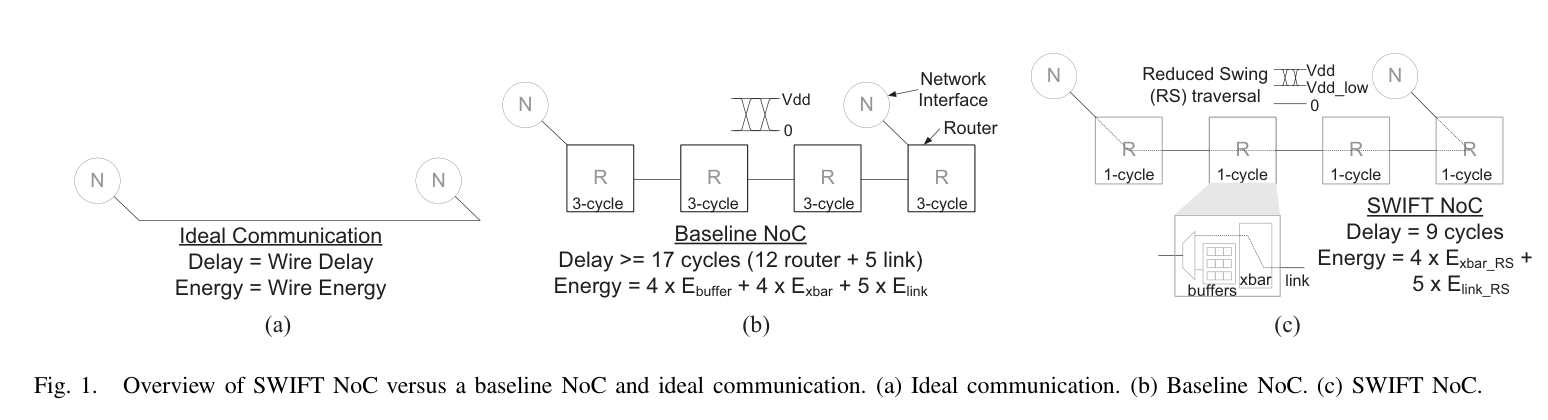
\includegraphics[width=0.88\textwidth]{chapters/ch02-switching-flow-control/figures/swift_fig01_overview.png}
\caption{Overview of SWIFT NoC versus baseline multi-stage NoC: (a) Ideal single-cycle communication, (b) Baseline multi-stage NoC, and (c) SWIFT NoC with token-based flit buffer bypassing. [Reproduced from: J. Postman, T. Krishna, C. Edmonds, L.-S. Peh, and P. Chiang, ``SWIFT: A Low-Power Network-On-Chip Implementing the Token Flow Control Router Architecture With Swing-Reduced Interconnects,'' \emph{IEEE Trans. Very Large Scale Integr. (VLSI) Syst.}, vol. 21, no. 8, pp. 1432--1446, Aug. 2013~\cite{Postman2013}. \copyright~2013 IEEE]}
\label{fig:ch2_swift_overview}
\end{figure}

\begin{figure}[t]
\sidecaption[t]
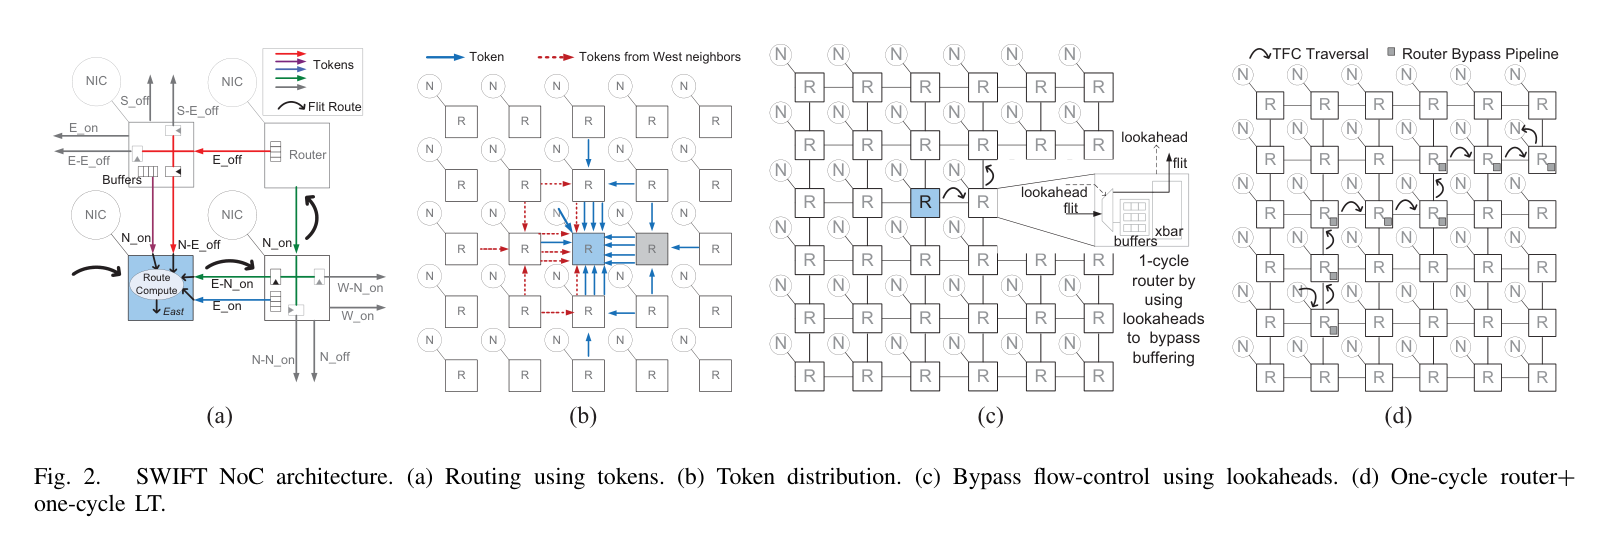
\includegraphics[width=0.65\textwidth]{chapters/ch02-switching-flow-control/figures/swift_fig02_token_flow.png}
\caption{SWIFT NoC microarchitecture: (a) Routing using tokens, (b) Token distribution, (c) Bypass flow control using lookahead signals, and (d) 1-cycle router plus 1-cycle link traversal. [Reproduced from: J. Postman et al., \emph{IEEE Trans. Very Large Scale Integr. (VLSI) Syst.}, Aug. 2013~\cite{Postman2013}. \copyright~2013 IEEE]}
\label{fig:ch2_swift_details}
\end{figure}

Key innovations of the SWIFT architecture include:
\begin{enumerate}
    \item \textbf{Flit Buffer Bypassing}: Tokens reserve crossbar paths in advance; data flits cut straight through the crossbar into the link without writing into input SRAM FIFO cells.
    \item \textbf{Buffer Power Reduction}: Dynamic FIFO write power is slashed by 38\% at saturation and 25\% at low load.
    \item \textbf{Swing-Reduced Interconnects}: Reduced-swing transceivers on physical links substantially diminish dynamic energy dissipation.
\end{enumerate}

\section{Interactive Lab \& Hands-on Challenges}
\label{sec:ch2_interactive}

Explore the interactive flow-control simulators on the \textbf{NoC Learning Hub} (\url{https://network-on-chip.github.io/learning/}):
\begin{itemize}
    \item \textbf{Credit Commander: Flow Control} (\url{https://network-on-chip.github.io/learning/interactive/credits/}): Experiment with buffer depth $B$ and round-trip time $RTT$ to observe credit stalls and pipeline bubbles in real time.
    \item \textbf{Packet Master: Routing Puzzle} (\url{https://network-on-chip.github.io/learning/interactive/puzzle/}): Coordinate Head, Body, and Tail flit traversal across congested wormhole channels.
\end{itemize}

\section{Checkpoint Assessment}
\label{sec:ch2_assessment}

\begin{enumerate}
    \item \textbf{Question 2.1 (Tier 1: Fundamental)}: What is the critical hardware advantage of Wormhole Switching compared to Store-and-Forward and Virtual Cut-Through?
    \item \textbf{Question 2.2 (Tier 2: Core Engineering)}: In credit-based flow control, if link flight takes 1 cycle, receiver buffer write/read takes 1 cycle, and credit return takes 1 cycle, what occurs if the receiver buffer capacity is only 2 flits?
    \item \textbf{Question 2.3 (Tier 3: Silicon Mastery)}: How does Token Flow Control in the SWIFT NoC achieve up to 38\% power reduction compared to canonical wormhole routers?
\end{enumerate}
\emph{Detailed answers and derivations for these questions are provided in the Solutions chapter at the end of this volume.}
